%
% gaussrand.tex
%
% (c) 2021 Prof Dr Andreas Müller, OST Ostschweizer Fachhochschule
%
\documentclass[tikz]{standalone}
\usepackage{times}
\usepackage{amsmath}
\usepackage{txfonts}
\usepackage[utf8]{inputenc}
\usepackage{graphics}
\usetikzlibrary{arrows,intersections,math}
\usepackage{ifthen}
\begin{document}

\newboolean{showgrid}
\setboolean{showgrid}{false}
\def\breite{7}
\def\hoehe{4}

\begin{tikzpicture}[>=latex,thick]
\clip (-6.4,-3.86) rectangle (6.2,4.0);

% Povray Bild
\node at (0,0) {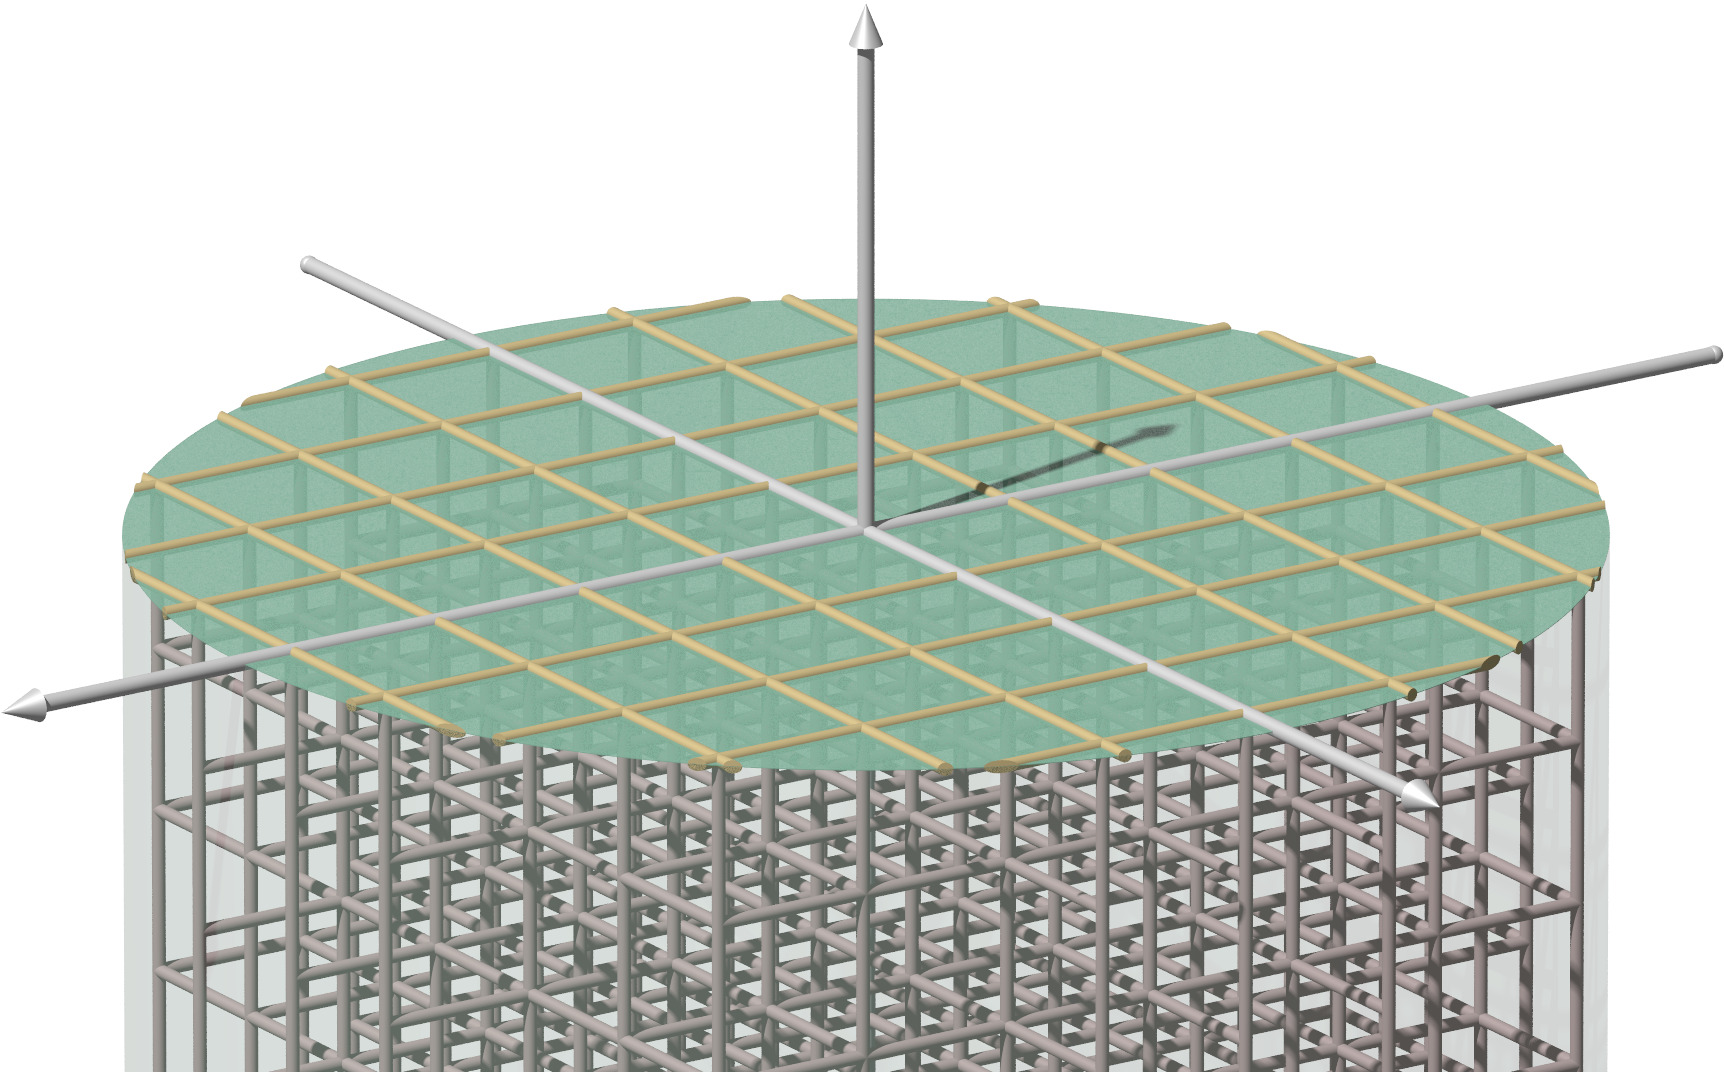
\includegraphics[width=12.4cm]{gaussrand.jpg}};

% Gitter
\ifthenelse{\boolean{showgrid}}{
\draw[step=0.1,line width=0.1pt] (-\breite,-\hoehe) grid (\breite, \hoehe);
\draw[step=0.5,line width=0.4pt] (-\breite,-\hoehe) grid (\breite, \hoehe);
\draw                            (-\breite,-\hoehe) grid (\breite, \hoehe);
\fill (0,0) circle[radius=0.05];
}{}

\node at (-6.2,-1) {$x^1$};
\begin{scope}[xshift=0.05cm]
\fill[color=white,opacity=0.7] (4.29,-1.71) circle[radius=0.22];
\node at (4.3,-1.7) {$x^2$};
\end{scope}
\node at (0.355,3.8) {$x^3$};
\node at (-1.5,0.4) {$\partial U_\alpha$};
\fill[color=white,opacity=0.7] (-0.5,-2.5) circle[radius=0.24];
\node at (-0.5,-2.5) {$U_\alpha$};

\end{tikzpicture}

\end{document}

